\chapter{Fallback skills e NLP}
\label{chap:fallback}
Sorge, dopo il lavoro svolto fino ad ora, un dubbio: cosa accadrebbe se la richiesta del paziente non fosse tra quelle previste durante la realizzazione della skill?
Le necessità mediche delle persone sono, purtroppo, ben più vaste di quanto si possa pensare di programmare. Viene quindi utile un approccio più "statistico", applicabile grazie alle più recenti scoperte nell'ambito dell'intelligenza artificiale.
\section{Classificazione del testo}
Esiste, nell'intelligenza artificiale, una branca che si occupa di \textbf{Natural Language Processing}, ossia processamento del linguaggio naturale. Vorremo quindi trovare un \textit{sistema} che approssimi al meglio la corrispondenza tra un input testuale ed un output che indichi una specifica classe. Il processo sarà quindi diviso in più parti: per primo, dovremo trovare un dataset testuale già categorizzato, o categorizzarne manualmente uno. Fatto ciò, dovremo trovare un modo di poter addestrare il computer a riconoscere i \textit{pattern} che legano un determinato testo alla sua classe d'appartenenza.
\section{Dataset utilizzato}
La presenza in rete di siti web come \textit{Kaggle} semplifica nettamente la ricerca di un dataset adatto alle necessità del data analyst. Purtroppo le moderne normative sulla privacy impongono la totale riservatezza dei dati medici delle persone. Esistono però, fortunatamente, dei dataset creati ad-hoc per la risoluzione di problematiche come quella qui presentata. Il dataset sfruttato per questa tesi\cite{dataset:medical-speech}, creato dalla \textbf{Appen}, azienda australiana specializzata in \textit{training data}, contiene audio, trascrizioni e intents di pazienti richiedenti aiuto. Tutto il dataset è in lingua inglese. Siccome la parte di Speech To Text viene gestita da Mycroft, utilizzeremo soltanto il dataset di trascrizioni ed intents. Ad esempio, alcune entries del dataset, potrebbero essere:
\begin{table}[H]
    \begin{tabularx}{\textwidth}{|l|X|}
        phrase: & My son had his lip pierced and it is swollen and the skin inside on his lip is grey and looks infected.
        \\
        prompt: & Infected wound
    \end{tabularx}
\end{table}
\begin{table}[H]
    \begin{tabularx}{\textwidth}{|l|X|}
        phrase: & I used to be out of breath after going up a dozen of stairs, but now I struggle to breath even when I sit down.
        \\
        prompt: & Hard to breath
    \end{tabularx}
\end{table}
\subsection{Traduzione del dataset}
\label{section:traduzione}
Siccome il bot deve funzionare anche in italiano, risulta evidente la necessità di una traduzione. Potremmo pensare di utilizzare le API di Google Translate, ma la traduzione di tutti i record del dataset (circa 8000), avrebbe un prezzo non indifferente. Si potrebbe quindi risolvere automatizzando l'utilizzo dell'interfaccia web tramite uno strumento come \textit{Selenium}. Fortunatamente, esistono già librerie Python per fare esattamente questo. Tra queste, \textbf{googletrans} è la più supportata dalla comunità.
Questa permette di definire un oggetto \texttt{Translator()} che sfruttiamo per la traduzione:
\begin{minted}{python}
for index, row in data.iterrows():
    phrase = translator.translate(row["phrase"], dest="it").text
    prompt = translator.translate(row["prompt"], dest="it").text
    if translator.detect(phrase).lang == "it" and translator.detect(prompt).lang == "it":
        translated_data.at[i, "phrase"] = phrase
        translated_data.at[i, "prompt"] = prompt
        i = i+1
\end{minted}
Quando Google Translate non riconosce il significato di una frase, non la traduce e la lascia come l'originale.
Notiamo che l'oggetto \texttt{translator} permette, oltre alla traduzione, di rilevare la lingua di una stringa. Questa caratteristica è d'aiuto per la realizzazione di un piccolo \textit{workaround} alle mancate traduzioni: se la funzione \texttt{detect} non rileva la lingua italiana sia nel testo che nella classe di appartenenza, la riga viene saltata. Questo riduce il numero di entries da circa 8000 a poco più di 2000. Gli esempi prima riportati sono ora:
\begin{table}[H]
    \begin{tabularx}{\textwidth}{|l|X|}
        phrase: & Mio figlio ha avuto il labbro trafitto ed è gonfio e la pelle all'interno del suo labbro è grigia e sembra infetta.
        \\
        prompt: & Ferita infetta
    \end{tabularx}
\end{table}
Notiamo qui che un piercing è diventato un \textit{labbro trafitto}, ma il senso generale è comunque ben chiaro.
\begin{table}[H]
    \begin{tabularx}{\textwidth}{|l|X|}
        phrase: & Ero senza fiato dopo aver salito una dozzina di scale, ma ora faccio fatica a respirare anche quando mi siedo.
        \\
        prompt: & Difficile da respirare
    \end{tabularx}
\end{table}
Anche qui, notiamo un piccolo problema di traduzione: le classi come \textit{"breathing difficulties"} vengono tradotte in modo letterale. Essendo però le classi in numero limitato, possiamo effettuare un \textit{find and replace}, passando, ad esempio, a \textit{Difficoltà respiratorie}.
\section{Addestramento della rete neurale}
Avendo ora un dataset in italiano, possiamo procedere con l'addestramento di una rete neurale che classifichi i testi. Per fare ciò, si è deciso di sfruttare la libreria \textbf{fastai}.
\subsection{fastai}
La libreria \textbf{fastai} semplifica il training e la creazione di reti neurali tramite le più recenti scoperte nell'ambito del deep learning. Tra le varie interfacce disponibili nella libreria, siamo interessati alla sezione riguardante il testo. Qui, è presente la classe \texttt{text.learner}, il cui scopo principale è addestrare un modello tramite il metodo \texttt{fit()}. Questa libreria permette inoltre di esportare suddetto modello, allo scopo di integrarlo in applicazioni senza dover effettuare il training ad ogni utilizzo. Esattamente quello che fa al nostro caso: possiamo addestrare la rete neurale una volta sola, ed utilizzare i risultati dell'addestramento a tempo indeterminato nell'assistente vocale, sostituendoli solo quando migliorati.
\subsection{Preparazione dei dati}
Una volta ottenuto il file CSV tradotto, effettuiamo l'importazione su Google Colab e li inseriamo in un dataframe per verificare l'assenza di NaN. Fatto ciò, possiamo creare una \texttt{TextList} di \textit{fastai}. Questo oggetto è un'\texttt{ItemList} specializzata nel testo, ossia una struttura di memoria che raggruppa gli input per il modello.
\begin{minted}[]{python}
path = Path('/content/')
data_clas = (TextList.from_csv(path, 'translations.csv', 
                            cols='phrase')
                .random_split_by_pct(.2)
                .label_from_df(cols='prompt')
                .databunch(bs=42))
\end{minted}
Fatto ciò, creiamo l'oggetto \texttt{text\_classifier\_learner}. Questo è basato su una Recurrent Neural Network. Scegliamo, come architettura, \texttt{AWD-LSTM}, che si è dimostrata vincente nella risoluzione di problemi di classificazione del testo simili a questo.
\subsubsection{AWD-LSTM}
Le Recurrent Neural Networks risolvono un problema fondamentale: se avessimo un input di dimensioni variabili, come potremmo creare un modello funzionale? Si potrebbe pensare di utilizzare più reti neurali classiche, ma non esisterebbe interazione tra gli input.
\begin{figure}[H]
    \begin{center}
        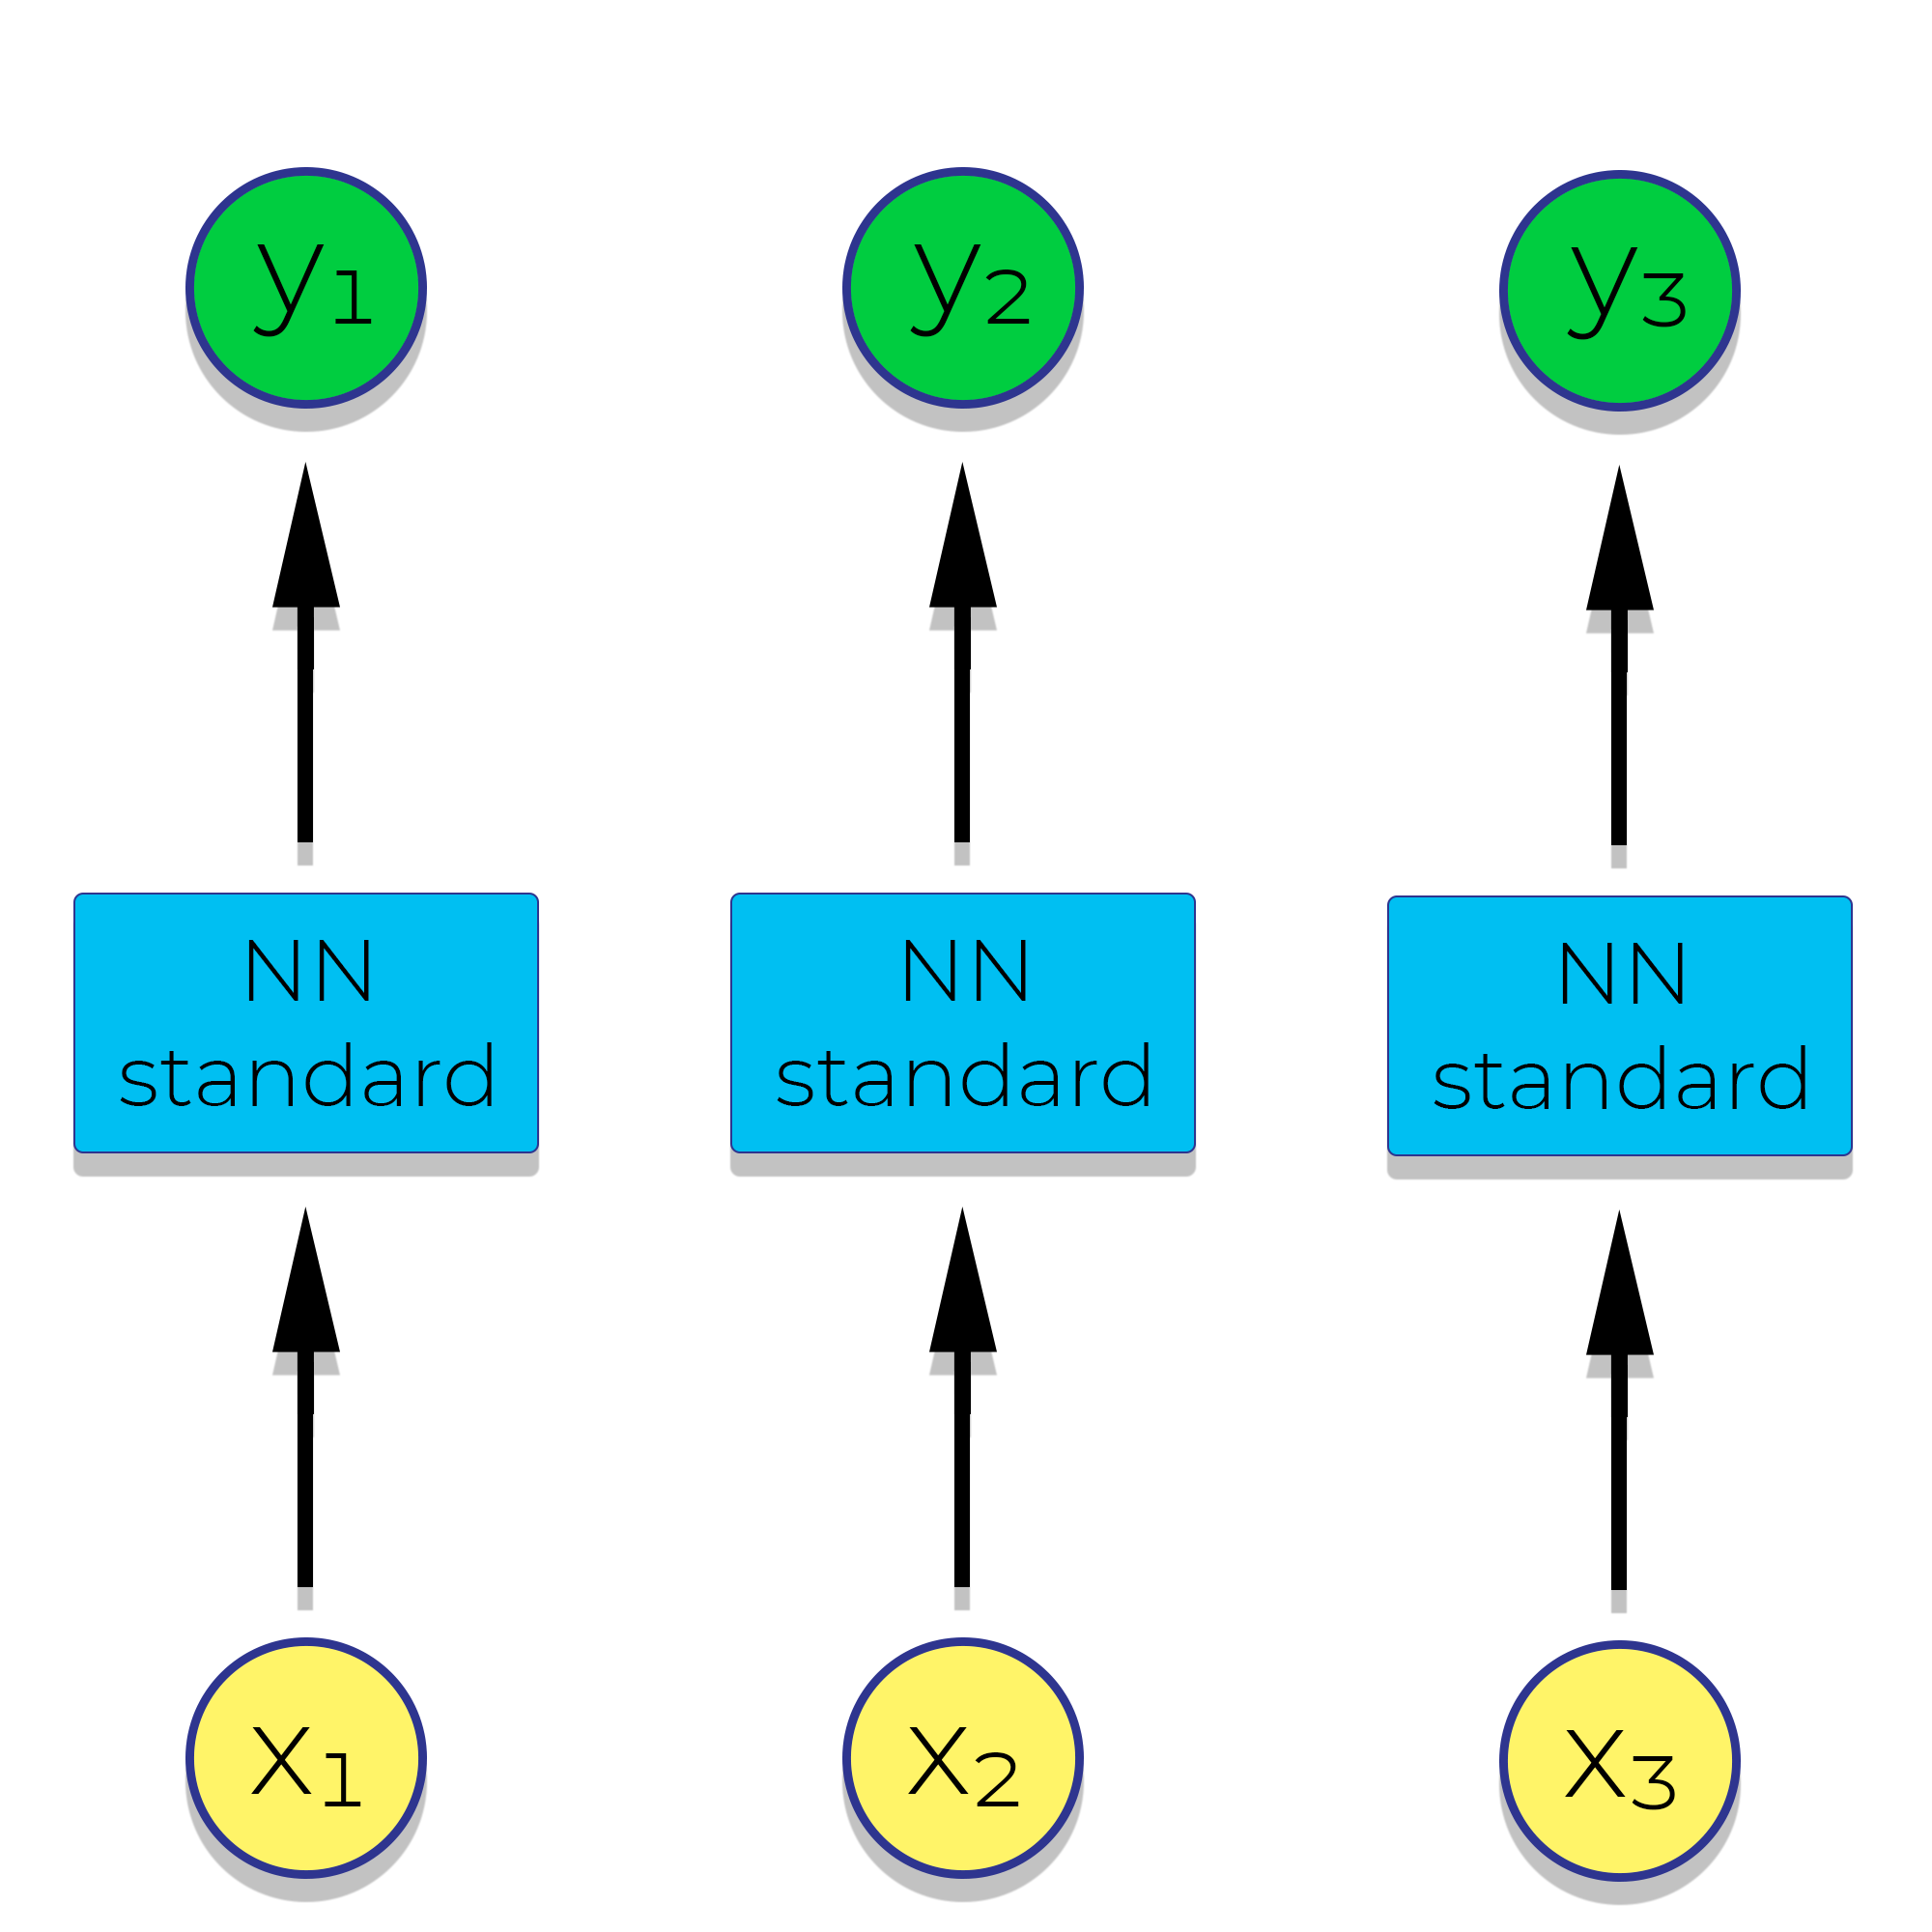
\includegraphics[width=0.5\columnwidth]{images/fallback/multiply-called-NN.png}
    \end{center}
    \caption{Reti neurali standard, chiamate più volte in base alla dimensione dell'input}
    \label{fig:multiply-called-NN}
\end{figure}
La soluzione portata dalle RNN è invece utilizzare come input di una rete neurale l'output della precedente. Questa caratteristica porta un vantaggio fondamentale: la rete ha ora \textit{memoria}, e l'output non dipende più solo dall'input singolo, ma da quelli precedenti.
\begin{figure}[H]
    \begin{center}
        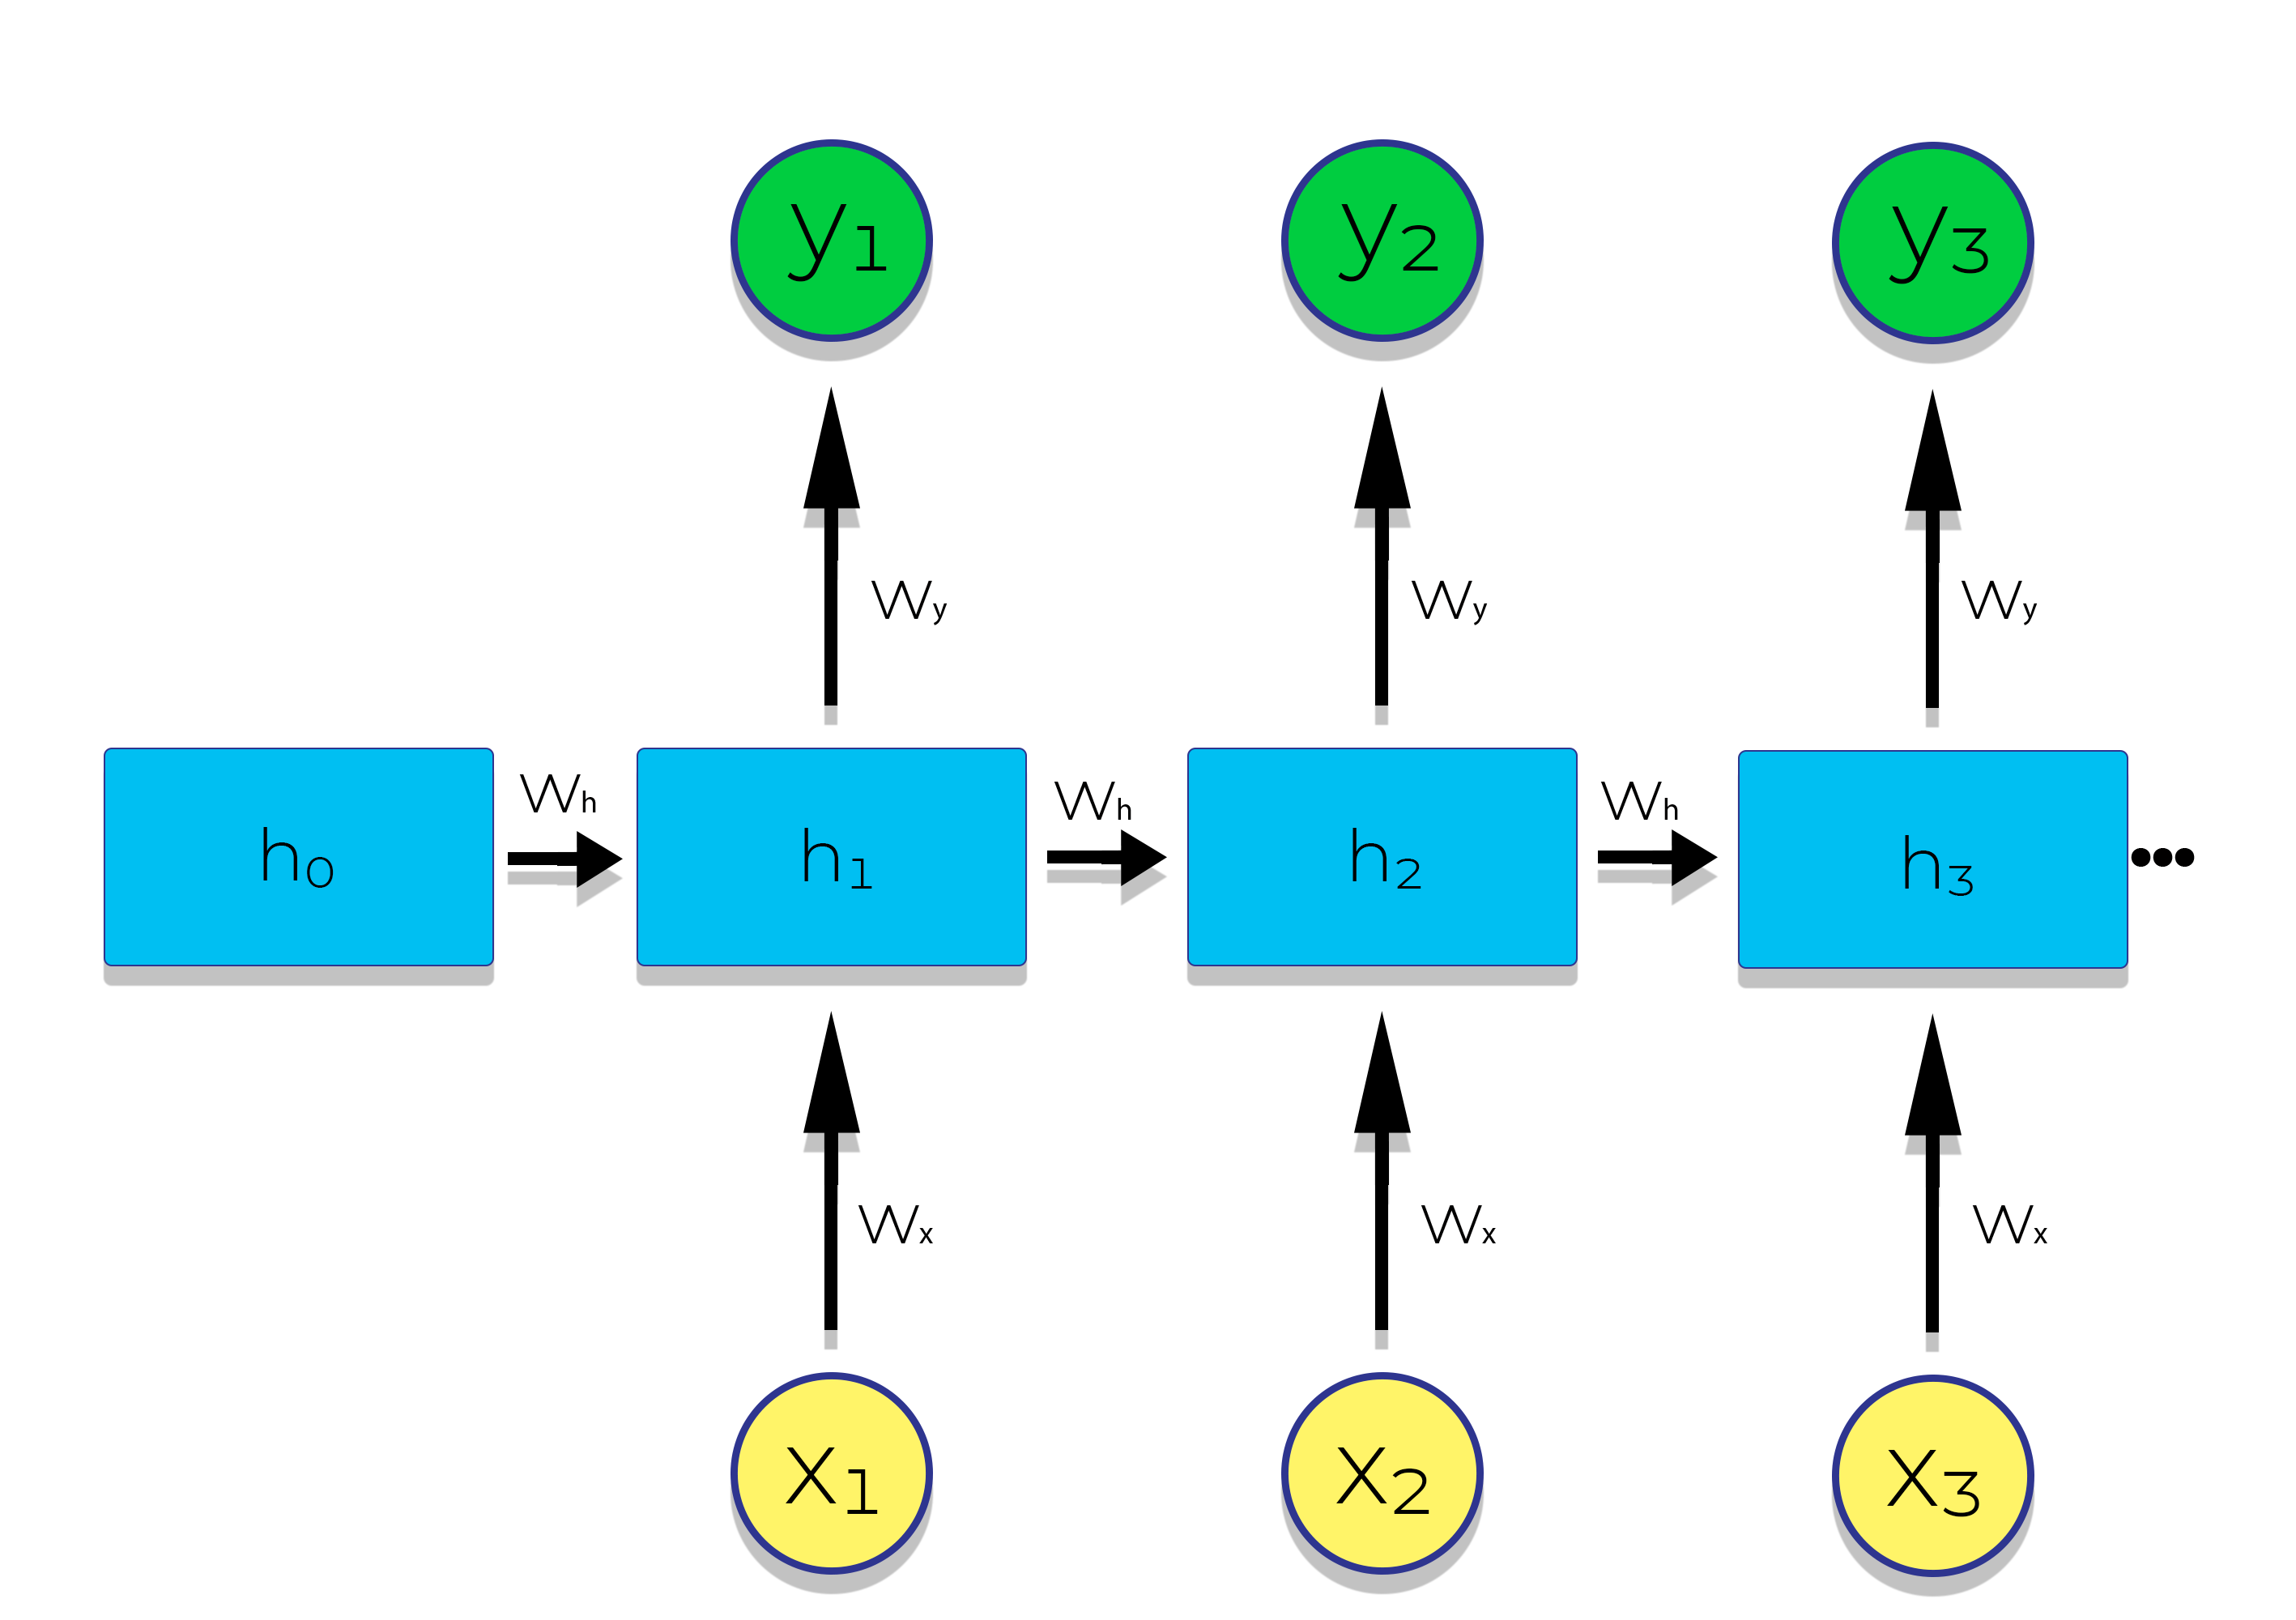
\includegraphics[width=0.5\columnwidth]{images/fallback/unfolded-RNN.png}
    \end{center}
    \caption{Recurrent Neural Network, aperta}
    \label{fig:unfolded-RNN}
\end{figure}
Considerando il peso $W_h$ sempre uguale, si ottiene lo schema consueto di RNN.
\begin{figure}[H]
    \begin{center}
        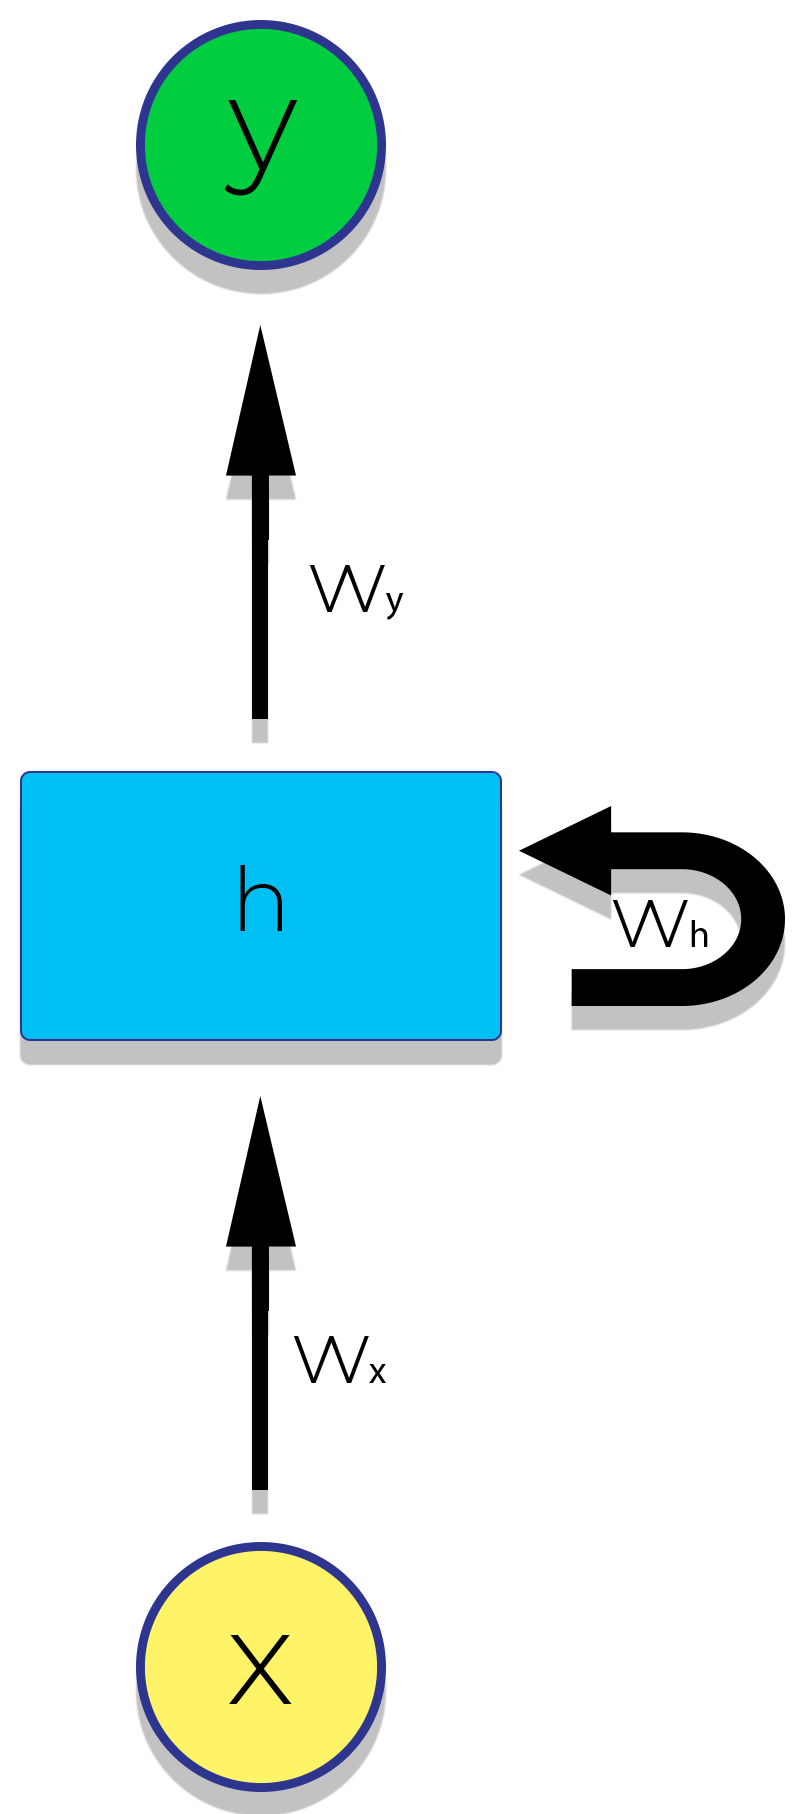
\includegraphics[width=0.3\columnwidth]{images/fallback/folded-RNN.png}
    \end{center}
    \caption{Recurrent Neural Network}
    \label{fig:folded-RNN}
\end{figure}
LSTM sta per \textit{Long Short Term Memory}. Questa tipologia di reti neurali estende il concetto di \textit{memoria a breve termine} delle RNN. A volte, la capacità di queste ultime di avere una \textit{memoria} è molto ridotta: se il gap tra informazioni utili è stretto, la memoria risulta sufficiente, altrimenti no. Le reti LSTM, introdotte da Hochreiter e Schmidhuber nel 1997\cite{paper:hochreiter1997long}, risolvono esattamente questo problema. Questo risultato viene raggiunto modificando la struttura interna delle singole reti neurali, più in particolare del modulo \textit{ripetente}, ossia quello che gestisce il passaggio della \textit{memoria} da una cella all'altra. Questa struttura, molto semplice nelle RNN standard (si tratta solamente di una $tanh$), diventa molto più complessa: la cella decide ora quali parti della memoria conservare, e quali sostituire con quelle derivate dal nuovo input. Le strutture di reti LSTM sono svariate, ma solitamente si basano su tre \textit{regolatori}, detti \textbf{gates}: l'\textit{input gate}, l'\textit{output gate} ed il \textit{forget gate}. AWD-LSTM (\textit{ASGD Weight-Dropped LSTM}) è una tipologia di reti neurali LSTM che fa utilizzo di \textit{DropConnect} (una particolare tipologia di Dropout che azzera i pesi al posto delle attivazioni) e ASGD (\textit{Average Stochastic Gradient Descent}), una versione dell'algoritmo di SGD che tiene conto di più interazioni piuttosto che di una sola.
\subsection{Addestramento della rete}
Addestriamo quindi la rete, e generiamo una confusion matrix, che permette di verificare quanto errate siano le classificazioni, e quali errori sono più ricorrenti.
\begin{figure}[H]
    \begin{center}
        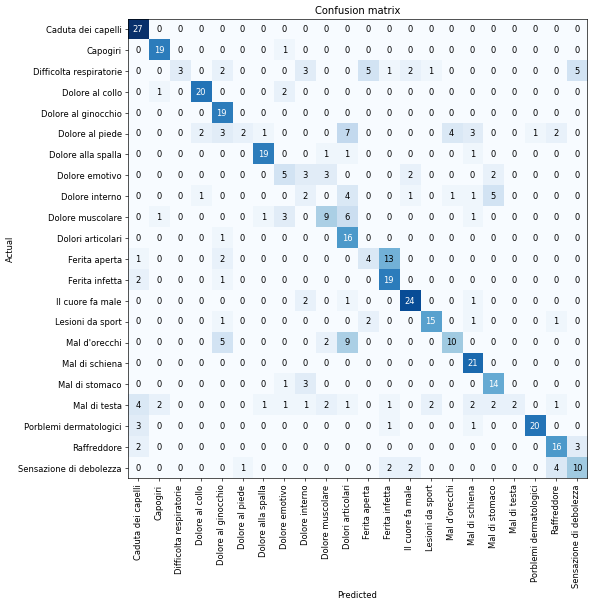
\includegraphics[width=0.8\columnwidth]{images/fallback/ConfusionMatrix.png}
    \end{center}
    \caption{Confusion Matrix}
    \label{fig:confusion-matrix}
\end{figure}
Notiamo il formarsi di una diagonale nella tabella: questo è sintomo di un \textbf{modello funzionante}. Possiamo quindi ora esportare il modello per l'utilizzo futuro.
\begin{minted}[]{python}
learn.export('/content/exported_model')
\end{minted}
Possiamo anche studiare l'accuracy nel corso delle varie epoche di training.
\begin{figure}[H]
    \begin{center}
        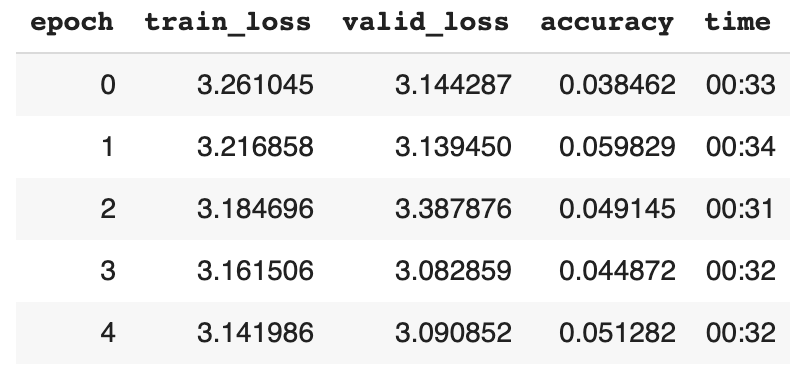
\includegraphics[width=0.5\columnwidth]{images/fallback/Accuracy.png}
    \end{center}
    \caption{Tabella delle accuracies}
    \label{fig:accuracy-table}
\end{figure}
Proviamo ora a predire la classe di una frase esempio, come "Sono caduto correndo":
\begin{minted}[]{python}
int(learn.predict("sono caduto correndo")[0])
\end{minted}
il risultato ottenuto è $15$, ossia la classe "Lesioni da sport".
\section{Realizzazione di fallback skills}
Come precedentemente spiegato, Mycroft funziona riconoscendo determinati \textit{intent} nelle richieste dell'utente. Questi sono stati da noi definiti nella skill del capitolo precedente. Abbiamo però specificato nell'introduzione che, a volte, i casi che abbiamo codificato non sono sufficienti:
\begin{enumerate}
    \item Svenimenti
    \item Emorragie
    \item Shock
    \item Difficoltà respiratorie
    \item Fratture
    \item Febbre
    \item Ustioni
    \item Dolori addominali
\end{enumerate}
Se si trattasse di una categoria esterna a queste, il paziente \textbf{non potrebbe venire aiutato}. Esiste però la possibilità di definire delle \textit{fallback skills}, ossia delle skill chiamate dall'assistente vocale quando la frase non viene riconosciuta dalle skill classiche. Queste hanno una priorità, e vengono chiamate nell'ordine definito da questa. Se una fallback skill riesce a risolvere la richiesta, non viene inoltrata alle altre. Vogliamo quindi ora creare un'automazione che sfrutti il modello ricavato dal natural language processing di cui sopra.
\subsection{Registrazione della skill}
La skill estende la classe \texttt{FallbackSkill}. Durante l'\textit{init} dell'oggetto, registriamo la fallback con una priorità di 10:
\begin{minted}[]{python}
self.register_fallback(self.handle_fallback, 10)
\end{minted}
Fatto ciò, possiamo caricare il modello di classificazione del testo precedentemente generato, assicurandoci che la libreria \textbf{fastai} sia installata.
\begin{minted}[]{python}
# Load the classifier model
self.learner = load_learner('models', 'exported_model')
# Load the classifier classes from JSON
with open('classes.json') as classes:
    self.classes = json.load(classes)
\end{minted}
Carichiamo inoltre il file \texttt{classes.json}, contenente le corrispondenze tra l'output numerico del modello e le classi testuali, oltre alle informazioni riguardanti la compatibilità del sintomo con il COVID19, l'immagine da mostrare nella GUI, e la gravità del sintomo:
\begin{minted}[]{json}
{
    "name": "Dolore al collo",
    "emoji": "[rimosso per motivi di stampa]",
    "code": "yellow",
    "covid": false
}
\end{minted}
Fatto ciò, resta da definire il comportamento del bot alla chiamata della fallback, operazione che svolgeremo con il metodo \texttt{handle\_fallback}.
Idealmente, questo dovrà predire la classe del sintomo, chiederne conferma al paziente, e aggiungere le informazioni alla scheda di triage.
\begin{minted}[]{python}
@symptom_handler
def handle_fallback(self, message):
    utterance = message.data.get("utterance")
    symptom = self.classes[int(self.learner.predict(utterance)[0])]
    self.gui.show_text(symptom["emoji"])
    did_i_get_that = self.ask_yesno(
        'symptoms.fallback', {"symptom": symptom["name"]})
    if did_i_get_that == "no":
        self.speak_dialog('sorry')
    else:
        if symptom["covid"]:
            self.ask_covid_questions()
        self.med_record["main_symptom"] = symptom["name"]
        self.med_record["code"] = symptom["code"]
\end{minted}
Ora il nostro bot, in caso di mancato riconoscimento del sintomo, potrà comunque indirizzare il paziente in modo automatizzato.
\section{Esempio di conversazione}
Riportiamo ora un esempio di conversazione realmente avvenuto.
\begin{itemize}
    \item \textbf{Utente:} \textit{Ho bisogno di aiuto}
    \item \textbf{Bot:} \textit{Lei è il paziente, non un accompagnatore, corretto?}
    \item \textbf{Utente:} \textit{Sì}
    \item \textbf{Bot:} \textit{Qual è il sintomo principale?}
    \item \textbf{Utente:} \textit{Mi è uscita la spalla mentre giocavo a golf}
    \item \textbf{Bot:} \textit{Trattasi quindi di dolore alla spalla, dico bene?}
    \item \textbf{Utente:} \textit{Esatto}
    \item \textbf{Bot:} \textit{Mi potresti dire quanti anni hai?}
    \item \textbf{Utente:} \textit{Ventidue}
    \item \textbf{Bot:} \textit{Se c'è qualche altro sintomo che devo sapere, dimmelo ora}
    \item \textbf{Utente:} \textit{Nient'altro}
    \item \textbf{Bot:} \textit{Come definirebbe il suo dolore da 1 a 10?}
    \item \textbf{Utente:} \textit{Sette}
    \item \textbf{Bot:} \textit{Potresti dirmi il tuo nome completo?}
    \item \textbf{Utente:} \textit{Mario Rossi}
    \item \textbf{Bot:} \textit{Il tuo nome è Mario Rossi, giusto?}
    \item \textbf{Utente:} \textit{Esatto}
    \item \textbf{Bot:} \textit{Grazie per la pazienza, recati al banco YELLOW}
\end{itemize}